% \documentstyle[amssymb,12pt,draft,epsf,palatino]{nature-pvd}
\documentclass{natureprintstyle}
\bibliographystyle{naturemag}

\usepackage{epsfig,caption}
\usepackage{color}
\usepackage{bm}
\usepackage{graphicx}
\usepackage{longtable}
\usepackage{amssymb}
\usepackage{rotating,xcolor}
\usepackage{hyperref}
\hypersetup{
    colorlinks,
    linkcolor={blue!50!black},
    citecolor={blue!80!white},
    urlcolor={blue!80!black}
}

\newcommand{\gyr}{\ensuremath{\textrm{Gyr}}}
\newcommand{\kpc}{\ensuremath{\textrm{kpc}}}
\newcommand{\mas}{\ensuremath{\textrm{mas}}}
\newcommand{\ul}{\ensuremath{\textrm{kpc}^2\,\textrm{Myr}^{-1}}}
\newcommand{\ue}{\ensuremath{\textrm{kpc}^2\,\textrm{Myr}^{-2}}}
\newcommand{\kms}{\ensuremath{\textrm{km}\,\textrm{s}^{-1}}}
\newcommand{\masyr}{\ensuremath{\textrm{mas}\,\textrm{yr}^{-1}}}
\newcommand{\feh}{\ensuremath{\textrm{[Fe/H]}}}
\newcommand{\afe}{\ensuremath{\textrm{[$\alpha$/Fe]}}}

\newcommand{\package}[1]{\textsl{#1}}

% \title{Signatures of Sagittarius rippling the entire Milky Way galaxy}
\title{Signatures of long-lived ripples throughout the Milky Way galaxy}

\author{Ana Bonaca$^1$, Rohan P. Naidu$^{2,3}$, Charlie Conroy$^4$}


\begin{document}

\maketitle

\let\thefootnote\relax\footnote{

\begin{affiliations}
\item The Observatories of the Carnegie Institution for Science, Pasadena, CA, USA

\item Massachusetts Institute of Technology, Cambridge, MA, USA
\item Hubble Fellow

\item Center for Astrophysics $|$ Harvard \& Smithsonian,  Cambridge, MA, USA

% \item Steward Observatory, University of Arizona, 933 North Cherry Avenue, Tucson, AZ 85721, USA
  
\end{affiliations}
}

\vspace{-3.5mm}
\begin{abstract}
Using a sample of $\sim16,000$ stars beyond the Milky Way's disk plane ($|Z_{gal}|\gtrsim2$\,kpc), we find evidence of discrete orbital resonances among the old stellar populations of the Milky Way. 
The resonances are present at similar orbital energy levels both in the high-latitude disk and in the radial halo components.
- recent: mw in disequilibrium
- here we show chaos super informative
(- check in sims / data if features more informative beyond the plane)
- measure where the peaks are
- kick off industry to constrain the locations of the peaks (test using chervin's models? share a notebook w the H3 selection function, potential we used)
\end{abstract}

\vspace{1cm}

%%%%%%%%%%%%%%%%%%%%%%%%%%%%%%%%%%%%%%%%%%%%%%%%%%%%%

We used optical spectroscopy from the ``Hectochelle in the Halo at High-resolution'' (H3) survey\cite{conroy:2019} to select $13,063$ high signal-to-noise ($\rm{SNR}>5$) giant stars ($\log g<3.5$, where $g$ is surface gravity).
The H3 survey targets are located in the northern sky ($\rm{Dec}>-20^\circ$), outside of the Milky Way disk plane ($|b|>30^\circ$) and at heliocentric distances larger than 2\,kpc.
The H3 pipeline\cite{} produces precise radial velocity measurements ($\sigma_{V_r}<1\lesssim1\,\kms$) and spectro-photometric distances 
Using proper motions from the Gaia Data Release 3\cite{}, and adopting the \package{astropy}v4.1 solar position\cite{}, we calculated 3D positions and 3D velocities for these stars.
- angular momentum wrt to the Galactic disk, and assuming MWPotential, total orbital energies with exquisite precision, median  (check amina's paper for phrasing of ELz)

\begin{figure*}
\begin{center}
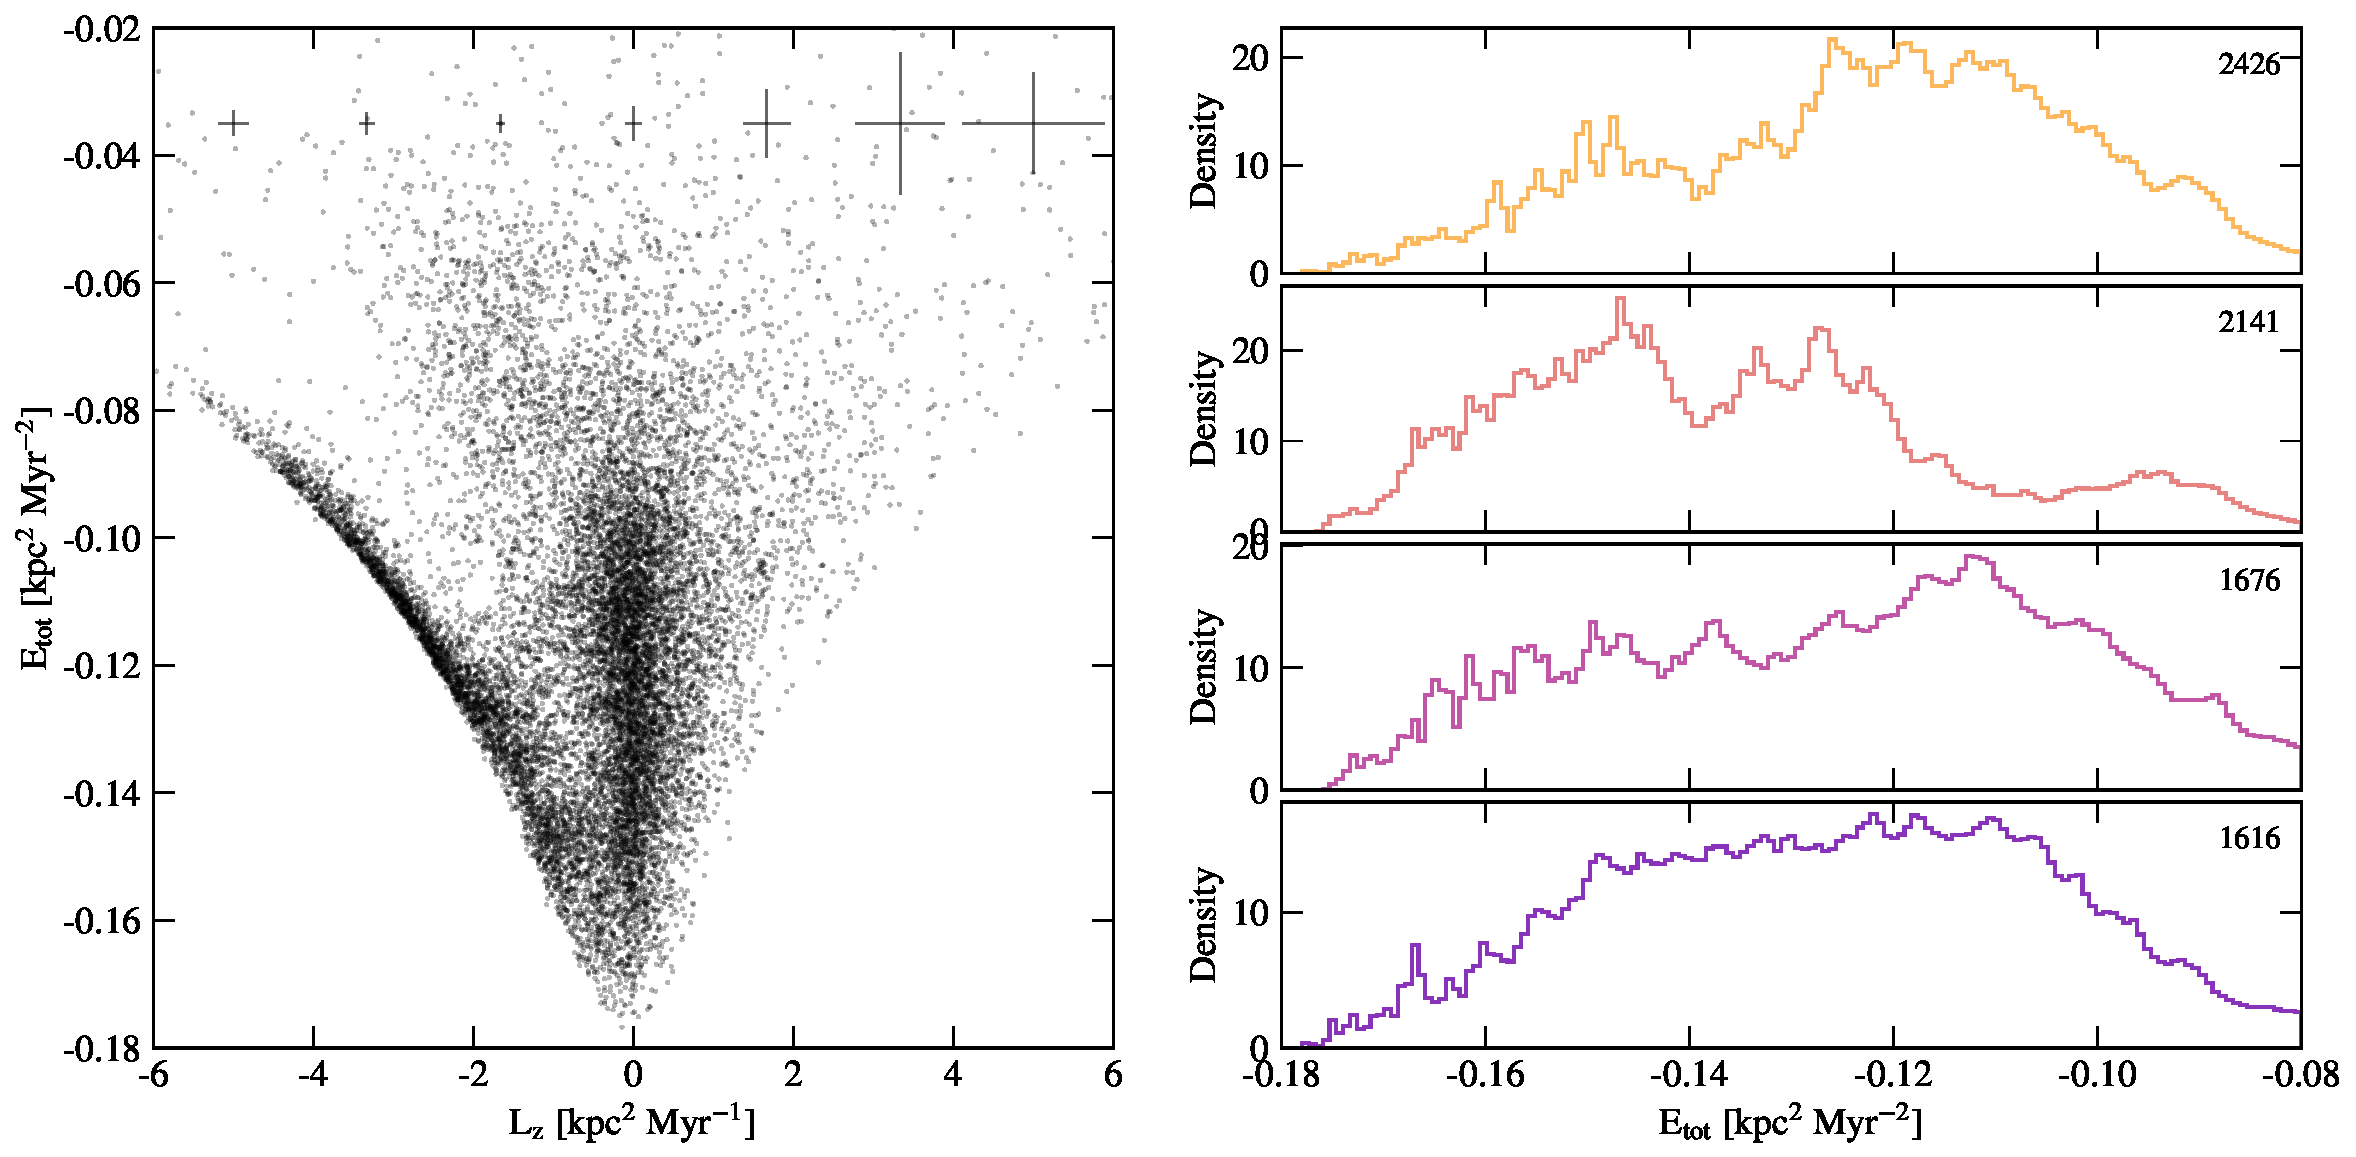
\includegraphics[width=0.95\textwidth]{fig1.pdf}
% \vspace{-4mm}
\caption{
\textbf{Orbital phase-space of Milky Way stars.}
{\bf Left panel:} Total orbital energies as a function of the $z$ component of orbital angular momentum (perpendicular to the Milky Way disk) of stars in the H3 survey.
Typical measurement uncertainties are shown as errorbars on top as a function of angular momentum.
- ripples
{\bf Right panels:} A resampled distribution of orbital energies, with each panel corresponding to a region of phase-space marked in the left panel.
The number of stars in each panel is indicated in the top right.
- best-fit model
}
% \vspace{-4mm}
\end{center}
\end{figure*}

- fig 1 shows E-Lz (2 panels: one points, another kde, annotated?)
- large scale clustering disk stars: left, GSE merger: center, retrograde shards: right, Sgr: top left + citations
- due to unprecedented precision (errorbars around the plot), we also detect small-scale clustering in the disk and the radial debris

- energy histograms (panel in fig 1)
- bootstraps
- fit mixture of gaussians
- auxiliary materials: non-bootstrapped version, function of snr; number of components

- why exciting: ringing -- disequilibrium easily mapped to dynamical history

- alternative: distinct accretion events
- smaller accretion events present, not obvious as overdensities\cite{naidu:2020}
- test through chemistry (fig 2)
- largely the same

- sim figure

- details of the simulation

- discrepancies

- comparison to other perturbations

- what we'll learn from this

%%%%%%%%%%%%%%%%%%%%%%%%%%%%%%%%%%%%%%%%%%%%%%%%%%%%

% \bibliographystyle{naturemag}
\bibliography{references}

\begin{addendum}
  
\item [Acknowledgements] 
% We thank both referees for their constructive
%   feedback.  C.C. is partially supported by the Packard
%   Foundation.  R.P.N. gratefully acknowledges an Ashford Fellowship
%   and Peirce Fellowship granted by Harvard University.  G.B.  and
%   N.G.-C. are supported by HST grant AR 15004, NASA ATP grant
%   17-ATP17-0006, NSF CAREER AST-1941096.  A.B. acknowledges support
%   from NASA through HST grant HST-GO-15930.  All the simulations were
%   run on El-Gato super computer which was supported by the National
%   Science Foundation under Grant No. 1228509.  We have made use of
%   data from the European Space Agency mission Gaia
%   (http://www.cosmos.esa.int/gaia), processed by the Gaia Data
%   Processing and Analysis Consortium (DPAC; see
%   http://www.cosmos.esa.int/web/gaia/dpac/consortium). Funding for
%   DPAC has been provided by national institutions, in particular the
%   institutions participating in the Gaia Multilateral Agreement.  This
%   publication makes use of data products from the {\it Wide-field
%     Infrared Survey Explorer}, which is a joint project of the
%   University of California, Los Angeles, and the Jet Propulsion
%   Laboratory/California Institute of Technology, and NEOWISE, which is
%   a project of the Jet Propulsion Laboratory/ California Institute of
%   Technology.  {\it WISE} and NEOWISE are funded by the National
%   Aeronautics and Space Administration.

\item[Author Contributions]
% C.C. and R.P.N. jointly conceived of the
%   project.  C.C. led the analysis of the data.  N.G-C. and
%   G.B. provided the simulation data and aided in its interpretation.
%   All authors contributed to aspects of the analysis and to the
%   writing of the manuscript.

\item[Author  Information]  
% Reprints and permissions
%     information is available at npg.nature.com/reprintsandpermissions.
%     Correspondence and requests for materials should be addressed to
%     C.C.\ (cconroy@cfa.harvard.edu).

\item[Data Availability] 
% The K giant catalog used in this paper is
%     available at \texttt{https://doi.org/10.7910/DVN/2D1H8J}.
    
\item[Code Availability] 
% We have opted not to make the code used in
%     this manuscript available because the data reduction and analysis
%     is straightforward and can be easily reproduced following the
%     methods described herein.
    
\end{addendum}


%%%%%%%%%%%%%%%%%%%%%%%%%%%%%%%%%%%%%%%%%%%%%%%%%%%%%%%%%%
%%%%%%%%%%%%%%%%%%%%%%%%%%%%%%%%%%%%%%%%%%%%%%%%%%%%%%%%%%

\newpage

\setcounter{page}{1}
\setcounter{figure}{0}
\setcounter{table}{0}
\captionsetup[figure]{labelformat=empty}
\renewcommand{\thefigure}{Extended Data \arabic{figure}}
\renewcommand{\thetable}{Extended Data \arabic{table}}

\begin{center}
{\bf \Large \uppercase{Methods}}
\end{center}

\noindent
{\bf Identification of giants}


\end{document}



